\chapter{Case study}
This chapter presents a case study where the load forecasting system is applied to Bruny Island.
As discussed in section \ref{scope} (\nameref{scope}), the aim of this case study is to develop a load forecasting system which can predict future load based on weather, holiday periods, car movement, and other factors. 
Bruny Island and the NAC will be used as a case study. 
The forecasting system is expected to be equally applicable to any power system network, \hl{and this will be demonstrated later in this chapter}.
\\
Specifically, the system will have the following properties:
\begin{itemize}
	\item The system will produce a forecast up to 24 hours in the future in 15- to 60-minute intervals. This will be a rolling forecast that can be re-calculated at any time.
	\item The forecast will be able to begin from any point time.
	\item The forecast will predict load in kVA at each interval.
	\item The forecast system will be aimed at predicting aggregate load at the feeder level. That is, between approximately 0.5 and 10MVA.
	\item The forecast system will be especially tuned to predict load during holiday periods.
\end{itemize}

\section{Bruny Island}
Bruny Island, shown in Figure \ref{fig:bruny_map}, is located approximately two kilometres off the coast of south-east Tasmania with a permanent resident population of approximately 800 people.
The island is a popular holiday destination, with Easter periods typically experiencing an influx of up to 500 cars in a single day.
The island is supplied by two feeders, depicted in Figure \ref{fig:bruny_network}, with  one feeder supplying a small portion of the island to the North and the other supplying the main portion of the island to the South.
This case study deals only with the feeder supplying the main portion of the island to the South.

During holiday period morning and afternoon peaks the submarine feeder reaches its capacity and a diesel generator located on the island is used to reduce the feeder load.
The substantial increase in load over the Easter holiday period for multiple years can be seen in Figure \ref{fig:bruny_easter}.

To avoid the use of the generator, the CONSORT project installed a set of residential batteries on the island for the purposes of peak-shifting.
These batteries are coordinated by the network aware coordination algorithm (NAC).
In order to peak-shift while making efficient use of the batteries, the NAC requires an accurate forecast of load with a 24-hour horizon and 30-minute resolution.
The proposed forecasting system was implemented for this purpose.

\begin{figure}[htbp]
	\centerline{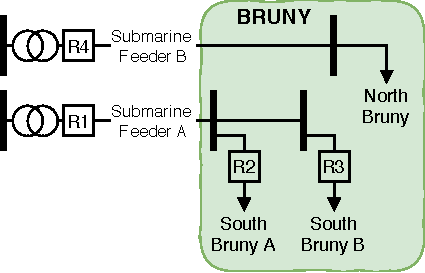
\includegraphics[width=.25\textwidth]{images/bruny_single_line.pdf}}
	\caption{Single line schematic of distribution network on Bruny Island.}
	\label{fig:bruny_network}
\end{figure}

\begin{figure}[htbp]
	\centerline{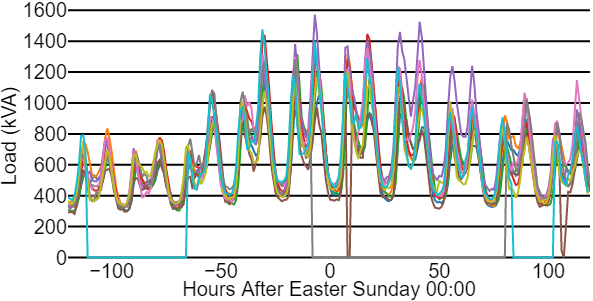
\includegraphics[width=.40\textwidth]{images/easter_bruny.png}}
	\caption{Easter load on Bruny Island 2008 through 2017.
		Unusable missing/bad data can also be seen in this graph.}
	\label{fig:bruny_easter}
\end{figure}

\subsection{Data and  Model Configuration}
The following data was available from 2009-2018:
\begin{itemize}
	\item Apparent power at reclosers R1 through R4 (Figure \ref{fig:bruny_network}).
	\item Temperature at Lenah Valley, Tasmania (50km from Bruny Island). 
	\item Apparent power consumption at St Helens, Tasmania.
\end{itemize}

This data was averaged to 30 minute resolution and split into a training set containing data from October 2009 through September 2014, and a testing set containing data from October 2014 through April 2018.

The network was supplied with data from the previous and future 24 hours, for a total input sequence length of 96 (representing 48 hours at 30 minute resolution).
The output sequence length was 48 (24 hours).

The following time series were supplied to the model input:
\begin{itemize}
	\item Apparent power from recloser R1 (Figure \ref{fig:bruny_network}), with future values set to zero.
	\item Temperature.
	\item Day of the week as an integer from 0 to 6 (local time).
	\item Minutes since midnight (local time).
	\item Boolean 1 or 0 indicating whether it is a holiday.
	\item Holiday type.
\end{itemize}

When used for inference, temperature forecasts were obtained from the Bureau of Meteorology.

Additionally, five similar periods were identified using data from R1 by the process described in section \ref{simperiod}.
The data over the similar periods for each of the following time series was provided as input:
\begin{itemize}
	\item Reclosers R1, R2, R3, and R4 (Figure \ref{fig:bruny_network}) (as separate time series).
	\item St Helens recloser.
	\item Lenah Valley temperature.
\end{itemize}

In total, 36 time series were provided as input to the model.
St Helens was included because it was observed to display similar patterns to Bruny Island around holiday periods.

The forecasting system was configured with the parameters in table \ref{table:parameters}, with the upper section giving transformer model parameters and the lower section giving weights used for similar period selection.

\begin{table}[htbp]
	\caption{Case study model parameters.}
	\begin{center}
		\begin{tabular}{clc}
			%			3.\hline
			\textbf{Parameter}&\textbf{Description}&\textbf{Value} \\
			\hline
			$L$ & Number of encoder and decoder layers & 4 \\
			$d$ & Hidden dimension & 32 \\
			$h$ & Number of attention heads & 4 \\
			$D$ & Dropout fraction & 0.2 \\
			$c$ & Loss function modifier & 3 \\
			-   & Training batch size & 16 \\
			\hline
			-   & Maximum future temperature weight & 10 \\
			-   & Minimum future temperature weight & 20 \\
			-   & Maximum past load weight & 30 \\
			-   & Holiday type weight & 1e9 \\
			-   & Day of week weight & 1e6 \\
			-   & Day of month weight & 1e6 \\
			-   & Month of year weight & 1e6 \\
			
		\end{tabular}
		\label{table:parameters}
	\end{center}
\end{table}

\subsection{Offline Evaluation}

The forecaster was first evaluated on historical data around Easter 2018, shown in Figure \ref{fig:easter_forecasts}.
Notably, the forecaster was able to accurately predict the first large peak while also transitioning smoothly between normal and holiday periods.
This is in contrast to load forecasting models which sometimes tend toward trivially repeating the previous day's load.


\begin{figure}[htbp]
	\centerline{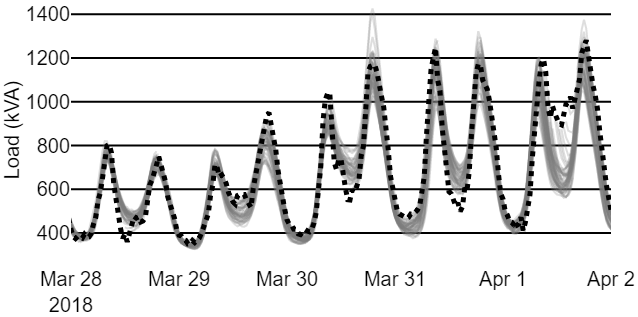
\includegraphics[width=.40\textwidth]{images/easter_2018_all_forecast.png}}
	\caption{Forecasts over the Easter 2018 period.
		The black dashed line is the actual recorded load, and all previous forecasts are shown in grey.}
	\label{fig:easter_forecasts}
\end{figure}

\begin{figure}[htbp]
	\centerline{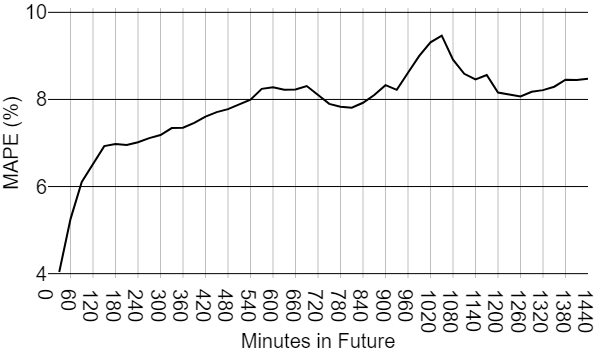
\includegraphics[width=.40\textwidth]{images/bruny_mape.png}}
	\caption{Mean absolute percentage error of each point in the forecast when evaluated over a variety of holiday periods.}.
	
	\label{fig:bruny_mape}
\end{figure}

The performance of the forecaster was evaluated on every Easter, Queen's Birthday, and July school holiday period from 2015 through 2018 (2018 excludes July).
The results are shown in Figure \ref{fig:bruny_mape}, showing the mean absolute percentage error (MAPE) as a function of forecast horizon.
The mean MAPE is 7.4\%.
Furthermore, the errors between predicted and actual load are fairly evenly distributed around -15 kVA, shown in Figure \ref{fig:bruny_hist}.
This indicates that the model has some room for improvement when predicting large holiday peaks, but overall this is evidence that the model has been able to generalize from the training data, as the training data is mostly comprised of normal days.

\begin{figure}[htbp]
	\centerline{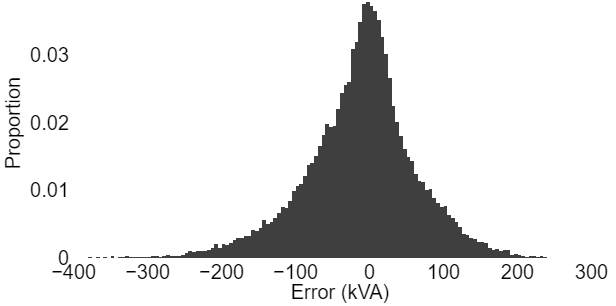
\includegraphics[width=.35\textwidth]{images/errors_histogram.png}}
	\caption{Distribution of forecast error when evaluated over the same periods as Figure \ref{fig:bruny_mape}.}
	\label{fig:bruny_hist}
\end{figure}

\subsection{Online Evaluation}
When implemented live on the Bruny Island distribution network during the July 2018 school holiday period, as part of the CONSORT project, the forecaster was observed to reliably forecast large demand peaks.
This enabled the fleet of distributed batteries to be used effectively in providing network support via net demand peak reduction. An accurate forecast, issued early enough in advance of the occurence of the demand peak, was observed to give the batteries adequate time to store energy in the lead up to, and discharge during the demand peak period. In at least one instance over the test period this was sufficient to avoid the island's diesel generator from being used at all, when it otherwise almost certainly would have been required.
Data collected during this peak demand period can be seen in Figure \ref{fig:bruny_nac}.
The upper section shows 24 hours of historical load in black, plus the most recent 24-hour horizon forecast in dashed black (recalculated every five minutes) and all old forecasts in grey.
The lower section shows the battery charge rate, where a negative value of battery charge rate indicates the batteries are supporting the grid.

Typically the generator is switched on when load exceeds 1050 kVA.
During the first peak the graph shows the batteries supplying between 50 and 100 kW to the island.
Without this support from the batteries, the generator would have been required to operate.

\begin{figure}[htbp]
	\centerline{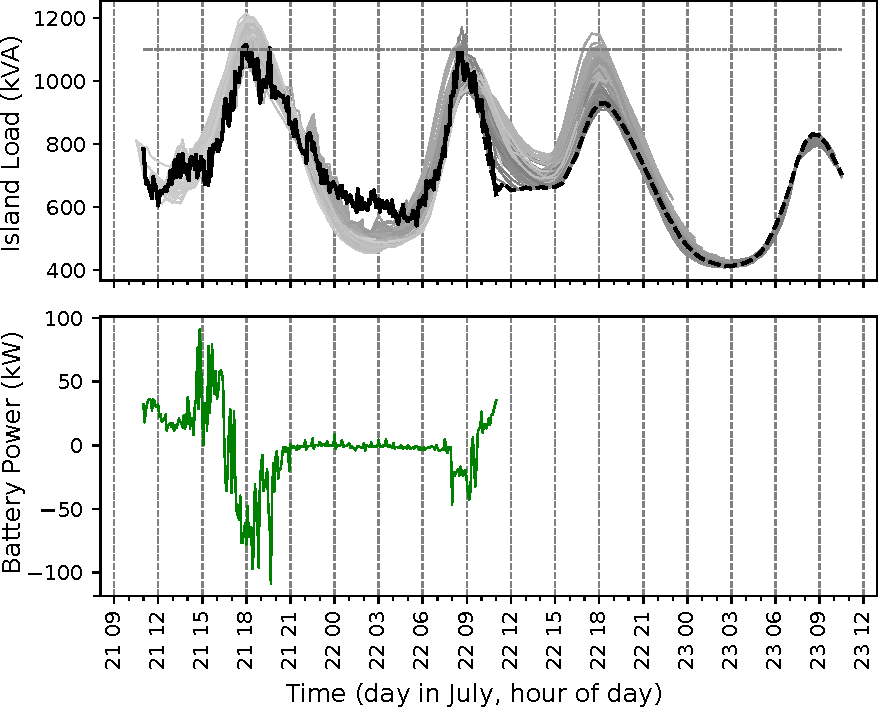
\includegraphics[width=.35\textwidth]{images/bruny_nac.pdf}}
	\caption{Results from the forecasting system's implementation in the CONSORT project.}
	\label{fig:bruny_nac}
\end{figure}



\subsection{Data analysis}
\label{bruny-data-analysis}
\hl{This section really rambles - it will be cut down a lot.}
\begin{itemize}
	\item \hl{this dot point list is for planning}
	\item discuss available data - load, weather, cars, other feeders and reclosers
	\item general load profiles of winter week, summer week, and full year
	\item look at annual growth of electricity. I need to investigate further my graph that is anomalous for 2013 and 2014 in growth.
	\item talk about different days of the week, and relate to car movement
	\item Look at special days - easter, june, christmas/ny
	\item talk about relationship between load and weather - temperature mainly
	\item Is load influenced by humidity like literature claims, or are temperature and humidity simply related?
	\item look at coloured scatter plot of load, temperature, and cumulative cars - more people correlates with more load in general - but we don't know future number of people.
	\item correlation matrix for power, cars, and weather
	\item cross correlations. Especially discuss any lags
	\item perhaps conclude with some important takeaways
	
\end{itemize}

In section \ref{patterns-profiles} the general properties of load profiles and how they are influenced by exogenous factors was discussed. Now, these general properties will be investigated in depth for the particular feeder in the case study.
\subsubsection{Available data}
The following data is available:
\todo[inline]{replace with a table}
\begin{itemize}
	\item kVA supplied through recloser R1 in 60 minute resolution between January 1, 2007 and March 9, 2012
	\item kVA supplied through recloser R1 in 5 minute resolution between March 9, 2012 and March 24, 2018
	\item kVA supplied to the feeder that R1 is connected to in 60 minute resolution between May 28, 2012 and March 24, 2018
	\item Ambient Temperature, solar irradiance, humidity, and wind speed at Lenah Valley between September 17, 2009 and March 24, 2018
	\item Vehicle movement data in 10 minute resolution between June 4, 2015 and March 24, 2018
\end{itemize}	
Vehicle movement data is provided as a set of observations every 10 minutes recording the number of vehicles arriving on the island, and the number of vehicles departing the island.
By integrating this, a relative number of vehicles on the island can be established.

There is a significant amount of bad or missing data throughout these datasets.
This has been handled by limiting the use of data where there are too many missing or bad values, as discussed later in this chapter.	


\subsubsection{Analysis}
Let's begin by having a simple look at some load profiles from the island.
Figure \ref{fig:load-profiles} shows apparent power draw on Bruny Island over a winter week, a summer week, and over an entire year.
These two weeks were selected to avoid special days such as holidays and are representative of typical weeks.
Some observations are immediately obvious
\begin{itemize}
	\item The midday load is only marginally larger than the overnight load in summer, but in winter it is significantly larger.
	\item Morning peaks are larger than afternoon peaks in summer, but in winter they are approximately equal.
	\item Thursday midday of the summer week appears abnormally high - perhaps this is a special day.
	\item There is some bad data on Tuesday of the summer week, as well as some missing data throughout the year.
	\item Over the whole year there appears to be a trend of increased max daily load over winter, which coincides with colder weather. This can be seen in the two individual weeks also.
	\item There are some periods of abnormally large load over the year: March 27, June 11, and December 28.
\end{itemize}

\begin{figure}[htbp]
	\centering
	\subfigure[]{
		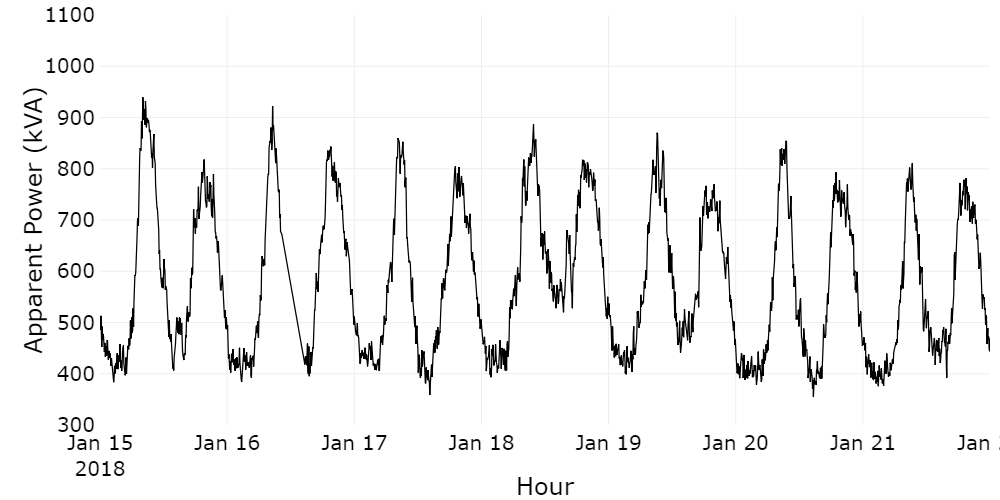
\includegraphics[width=0.8\textwidth]{images/simple-week-summer}
		\label{fig:simple-week-summer}}
	\vfil
	\subfigure[]{
		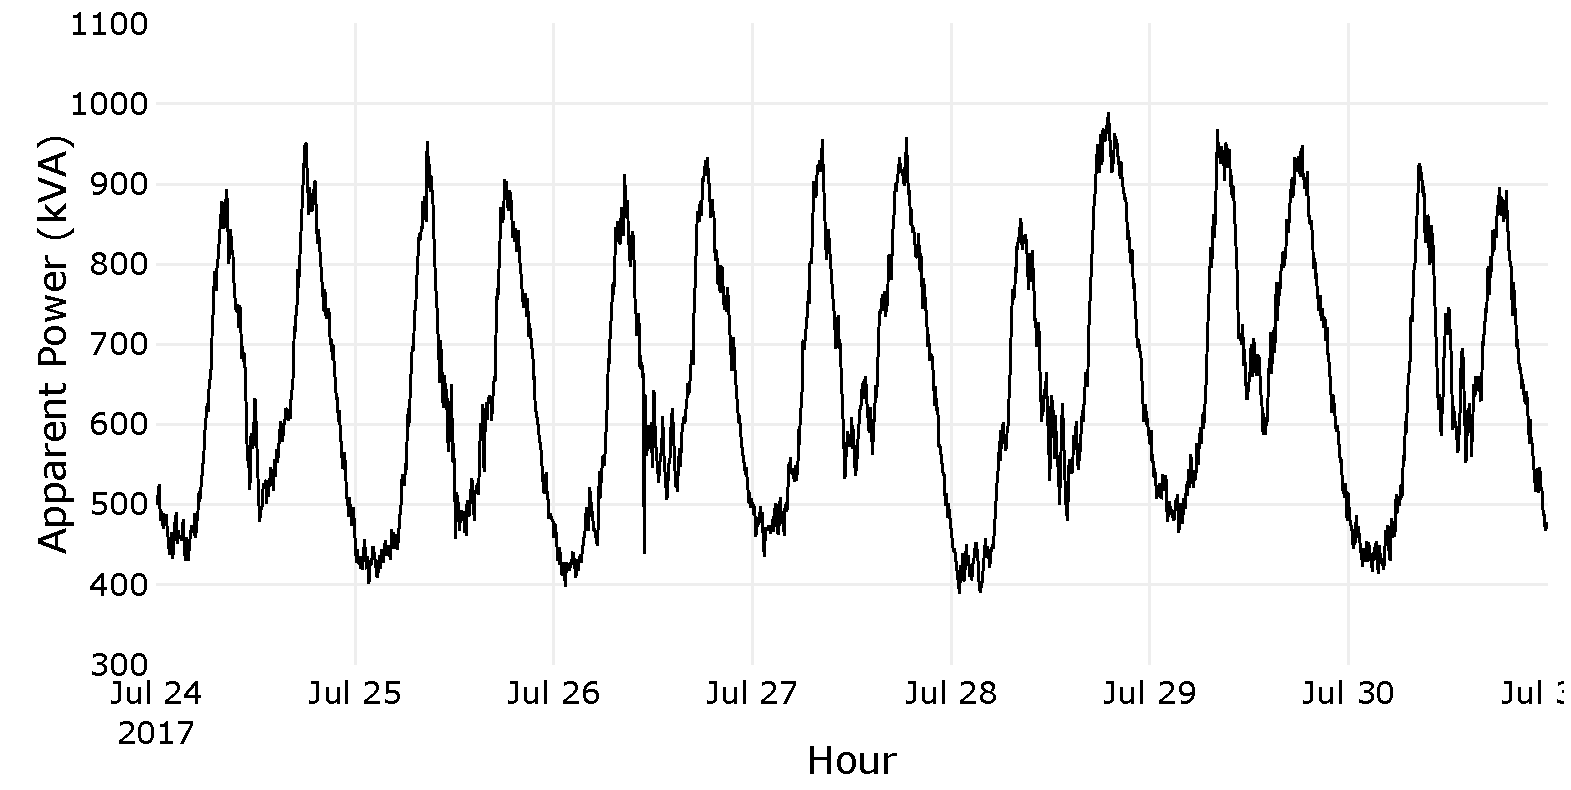
\includegraphics[width=0.8\textwidth]{images/simple-week-winter}
		\label{fig:simple-week-winter}}
	\vfil
	\subfigure[]{
		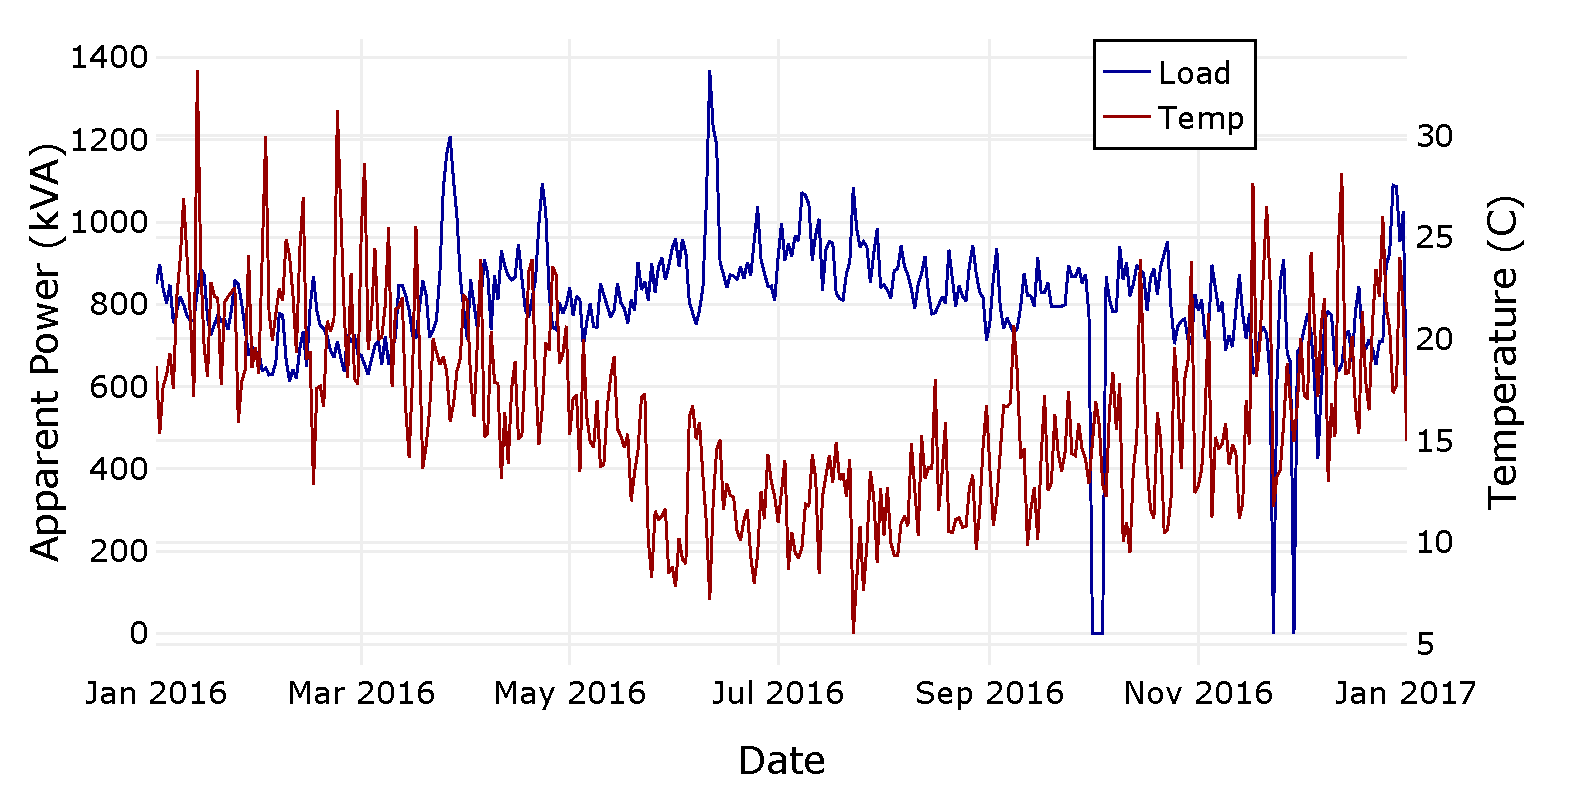
\includegraphics[width=0.8\textwidth]{images/max-load-max-temp}
		\label{fig:max-load-max-temp}}
	\caption{Bruny Island load profiles. (a) Load over a single summer week in 2018. (b) Load over a single winter week in 2017. (c) Peak daily load and peak daily temperature over all of 2017.}
	\label{fig:load-profiles}
\end{figure}

It was mentioned in section \ref{patterns-profiles} that weekends and weekdays tend to have different load profiles, but this is not immediately obvious from figure \ref{fig:load-profiles}.
Figure \ref{fig:average-profiles} shows this difference between days of the week.
What is immediately obviously is that the differences between days of the week are not restricted to 24 hour bounds - the different load profile shapes gently merge into each other over the course of an afternoon or morning.
% This is an especially important observation for a forecasting system that needs to be able to perform forecasts not just at a single time each day, but at any time.
It can be seen that the Friday profile morphs into the Saturday profile during the afternoon, perhaps as people arrive on the island for the weekend, and the Sunday profile morphs into a weekday profile over the afternoon, perhaps as people depart the island.

Figures \ref{fig:average-arriving} and \ref{fig:average-departing} further support that the changes in load profiles are a result of people arriving on or leaving the island.
It can be seen that many vehicles tend to arrive on the island on Friday afternoon, leading to the change in load profile between Friday and Saturday.
Likewise, many vehicles leave the island on Sunday afternoon, shifting the load profile from Sunday to a weekday.

%This observation, that the load profiles on weekends and weekdays are only partially different, could indicate that information may be lost by considering only a single day.

\begin{figure}[htbp]
	\centering
	\subfigure[]{
		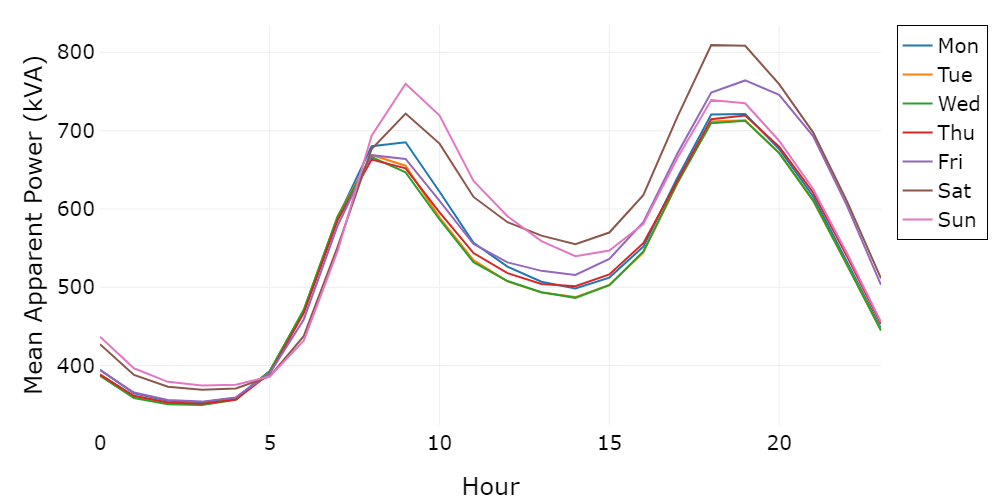
\includegraphics[width=.8\textwidth]{images/average-profiles}
		\label{fig:average-profiles}}
	\vfil
	\subfigure[]{
		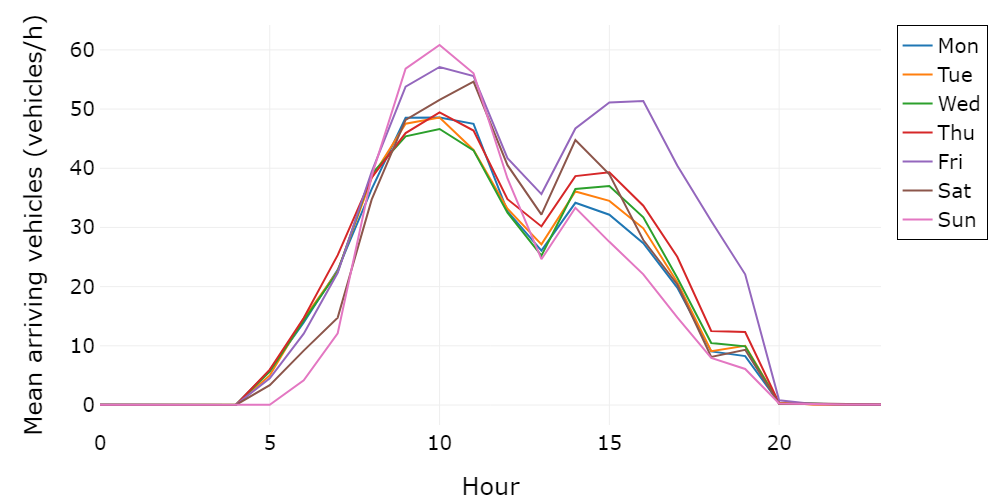
\includegraphics[width=.8\textwidth]{images/average-arriving}
		\label{fig:average-arriving}}
	\vfil
	\subfigure[]{
		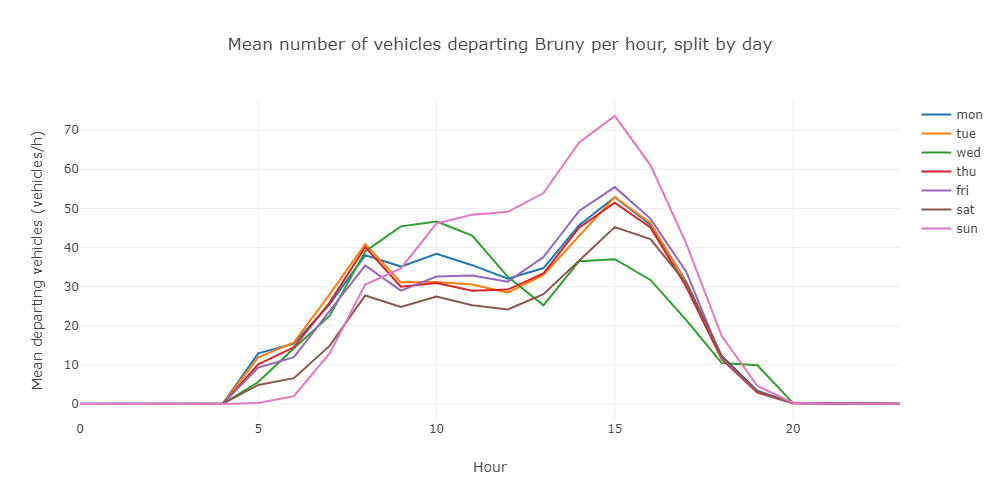
\includegraphics[width=.8\textwidth]{images/average-departing}
		\label{fig:average-departing}}
	\caption{Bruny Island average load profiles. (a) Average load profiles for each day of the week. Average number of cars arriving on (b) and leaving (c) the island each day.}
	\label{fig:average-load-profiles}
\end{figure}

Naturally, the next step is to attempt to look for clusters in the load profiles.
Looking at figure \ref{fig:all-monday-profiles}, there are no immediately obvious clusters.
However, it should be noted how the load profiles overnight have much lower variance than during the day - this will be important when evaluating the performance of the forecasting system if different models are used to forecast different hours of the day.

\begin{figure}
	\centering
	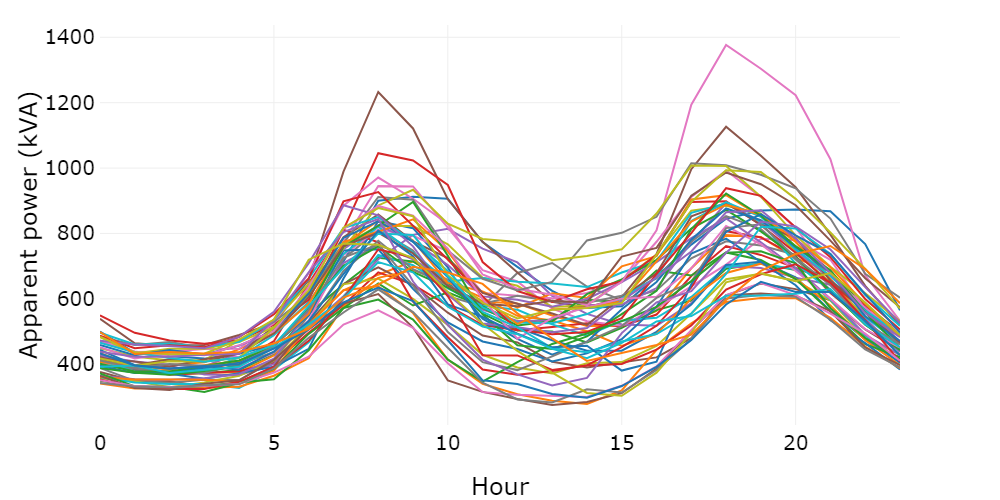
\includegraphics[width=0.8\linewidth]{images/all-monday-profiles}
	\caption{Load profiles of every Monday of 2017 overlaid. Notably, no clusters are immediately apparent in this plot.}
	\label{fig:all-monday-profiles}
\end{figure}
